% label prefix for this part: pm
\part{Projektmanagement}

\chapter{Vorgehensmodell}
Als Vorgehensmodell für die \acl{ba} wurde Scrum verwendet. Scrum ist ein agiles, iteratives Modell, welches sich aufgrund dessen Einfachheit und nicht besonders strikter Vorgaben sehr gut für kleinere, gut überschaubare Projekte eignet. Scrum basiert wie viele andere agile Projektmanagementmethoden auf den vier Grundsätzen die im Agilen Manifest~\cite{agilemanifesto} beschrieben sind:

\begin{itemize}
	\item Individuals and interactions over processes and tools
	\item Working software over comprehensive documentation
	\item Customer collaboration over contract negotiation
	\item Responding to change over following a plan
\end{itemize}

Wobei der Punkt \blockquote{Working software over comprehensive documentation} aufgrund der Tatsache, dass es sich um eine akademische Arbeit handelt, vernachlässigt wird.

\section{Rollen}
\mytable{lX}{
	\textbf{Rolle}  & \textbf{Beschreibung}\\
	\midrule
	
	\textbf{Product Owner} & Der Product Owner bestimmt die Anforderungen (User Stories) und priorisiert diese. Die Priorität gibt an, welche User Stories es im nächsten Sprint zu erledigt gilt.\\
	
	\textbf{Team} & Das Team besteht aus allen für das Projekt tätige Entwickler.\\
	
	\textbf{Scrum Master} & Der Scrum Master kümmert sich um die fortlaufende Kontrolle des Fortschritts sowie Optimierungsmöglichkeiten. In der Praxis ist er zudem für die Leitung der Daily Scrum Meetings, welche in diesem Projekt wegfallen, zuständig.\\
}{Scrum Projektrollen}{scrum-roles}

\section{Artefakte}
\mytable{lX}{
	\textbf{Artefakt}  & \textbf{Beschreibung}\\
	\midrule
	
	\textbf{Product Backlog} & Der Product Backlog enthält alle noch nicht abgeschlossenen User Stories des Projekts. Vor Beginn des neuen Sprints werden die noch offenen User Stories vom Product Owner repriorisiert und dessen Aufwand vom Team geschätzt.\\
	
	\textbf{Sprint Backlog} & Der Sprint Backlog enthält alle für einen bestimmten Sprint ausgewählte User Stories. Das Team setzt die Quantität fest und der Product Owner bestimmt den Inhalt und somit welche User Stories in den nächsten Sprint einfliessen.\\
	
	\textbf{Burndown Charts} & Mittels Jira werden laufend die Ist- und Sollstunden des Sprints addiert und daraus ein regressives Diagramm erstellt. Dies soll aufzeigen wie man zeitlich steht um mögliche Zeitprobleme zu vermeiden.\\
}{Scrum Artefakte}{scrum-artifacts}

\section{Sprints}

Die Iterationen, bei Scrum Sprint genannt und in \cref{fig:scrum} dargestellt, dauerten mit Ausnahme der ersten Woche jeweils zwei Wochen. So konnte, wie bei Scrum üblich, zum Ende jedes Sprints ein Deliverable, sei es eine lauffähige Applikation oder ein anderes Resultat, zur Verfügung gestellt werden.

\begin{figure}[H]
	\centering
	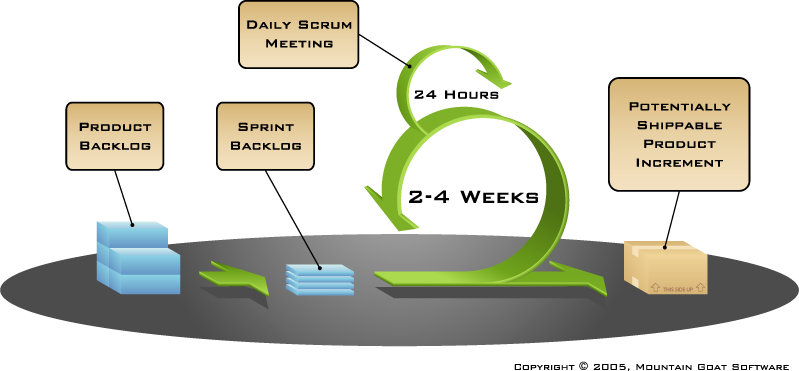
\includegraphics[width=0.7\linewidth]{fig/scrum}
	\caption[Scrum Sprint]{Scrum Sprint \cite{scrum}}
	\label{fig:scrum}
\end{figure}


\chapter{Rollen und Verantwortlichkeiten}

\section{\proff}

\begin{minipage}[t]{0.25\textwidth}
	\vspace{0pt}
	
\includegraphics[width=0.8\textwidth]{fig/sfkeller}
\end{minipage}
\begin{minipage}[t]{0.8\textwidth}
	\vspace{0pt}
	\prof, Mitarbeiter des \gls{ifs} und Dozent an der \gls{hsr} übernimmt im Projekt eine Doppelrolle:
	\begin{itemize}
		\item Als Experte bzw. Betreuer übernimmt er eine die Aufsicht und Bewertung der \acl{ba}
		\item und als fiktiver Kunde die Kontaktperson zur Aufnahme der Anforderungen (Product Owner).
	\end{itemize}
\end{minipage}


\section{\rlif}
\xxx[remo]
\begin{minipage}[t]{0.25\textwidth}
	\vspace{0pt}
	%\includegraphics[width=0.8\textwidth]{fig/rliebi}
\end{minipage}
\begin{minipage}[t]{0.8\textwidth}
	\vspace{0pt} 
	\rlif, Teilzeitstudent an der \gls{hsr}, Inhaber von der IT-Firma liebi.net, ist Teil des Entwicklungsteams.
\end{minipage}

\section{\chuf}
\begin{minipage}[t]{0.25\textwidth}
	\vspace{0pt}
	
\includegraphics[width=0.8\textwidth]{fig/chuesler}
\end{minipage}
\begin{minipage}[t]{0.8\textwidth}
	\vspace{0pt}
	\chuf, Vollzeitstudent an der \gls{hsr}, JavaEE-Entwickler und Datenbank-Experte bei Xinventa GmbH, ist Teil des Entwicklungsteams.
\end{minipage}


\section{\fscf}
\begin{minipage}[t]{0.25\textwidth}
	\vspace{0pt}
	
\includegraphics[width=0.8\textwidth]{fig/fscala}
\end{minipage}
\begin{minipage}[t]{0.8\textwidth}
	\vspace{0pt}
	\fscf, Teilzeitstudent an der \gls{hsr} und Banking Software Engineer bei Swisscom IT Serivces, ist Teil des Entwicklungsteams und übernimmt zusätzlich die Rolle des Scrum Masters.
\end{minipage}

\chapter{Risiken}\label{sec:risiken}

Für die Abschätzung der Projektrisiken wurde auf existierende \cite{risk} Risikochecklisten gesetzt um möglichst keine potenziellen Risiken bei der Analyse auszulassen. Die sehr umfangreiche Risikoliste von \citeauthor{Wallace:2004:SPR:975817.975819} \cite{Wallace:2004:SPR:975817.975819} wurde mit den bekannten Top Zehn Software-Projektrisiken aus dem Jahre \citeyear{boehm} \cite{boehm} sowie mit eigenen, Projektspezifischen Risiken ergänzt.
Auch die aus der Sicht des Teams, für das Projekt nicht relevante Risiken, wurden protokolliert und gelten als Nachweis, dass auch diese miteinbezogen und nicht etwa ignoriert oder gar vergessen wurden.

\begin{landscape}
	\begin{table}[H]
		\centering
		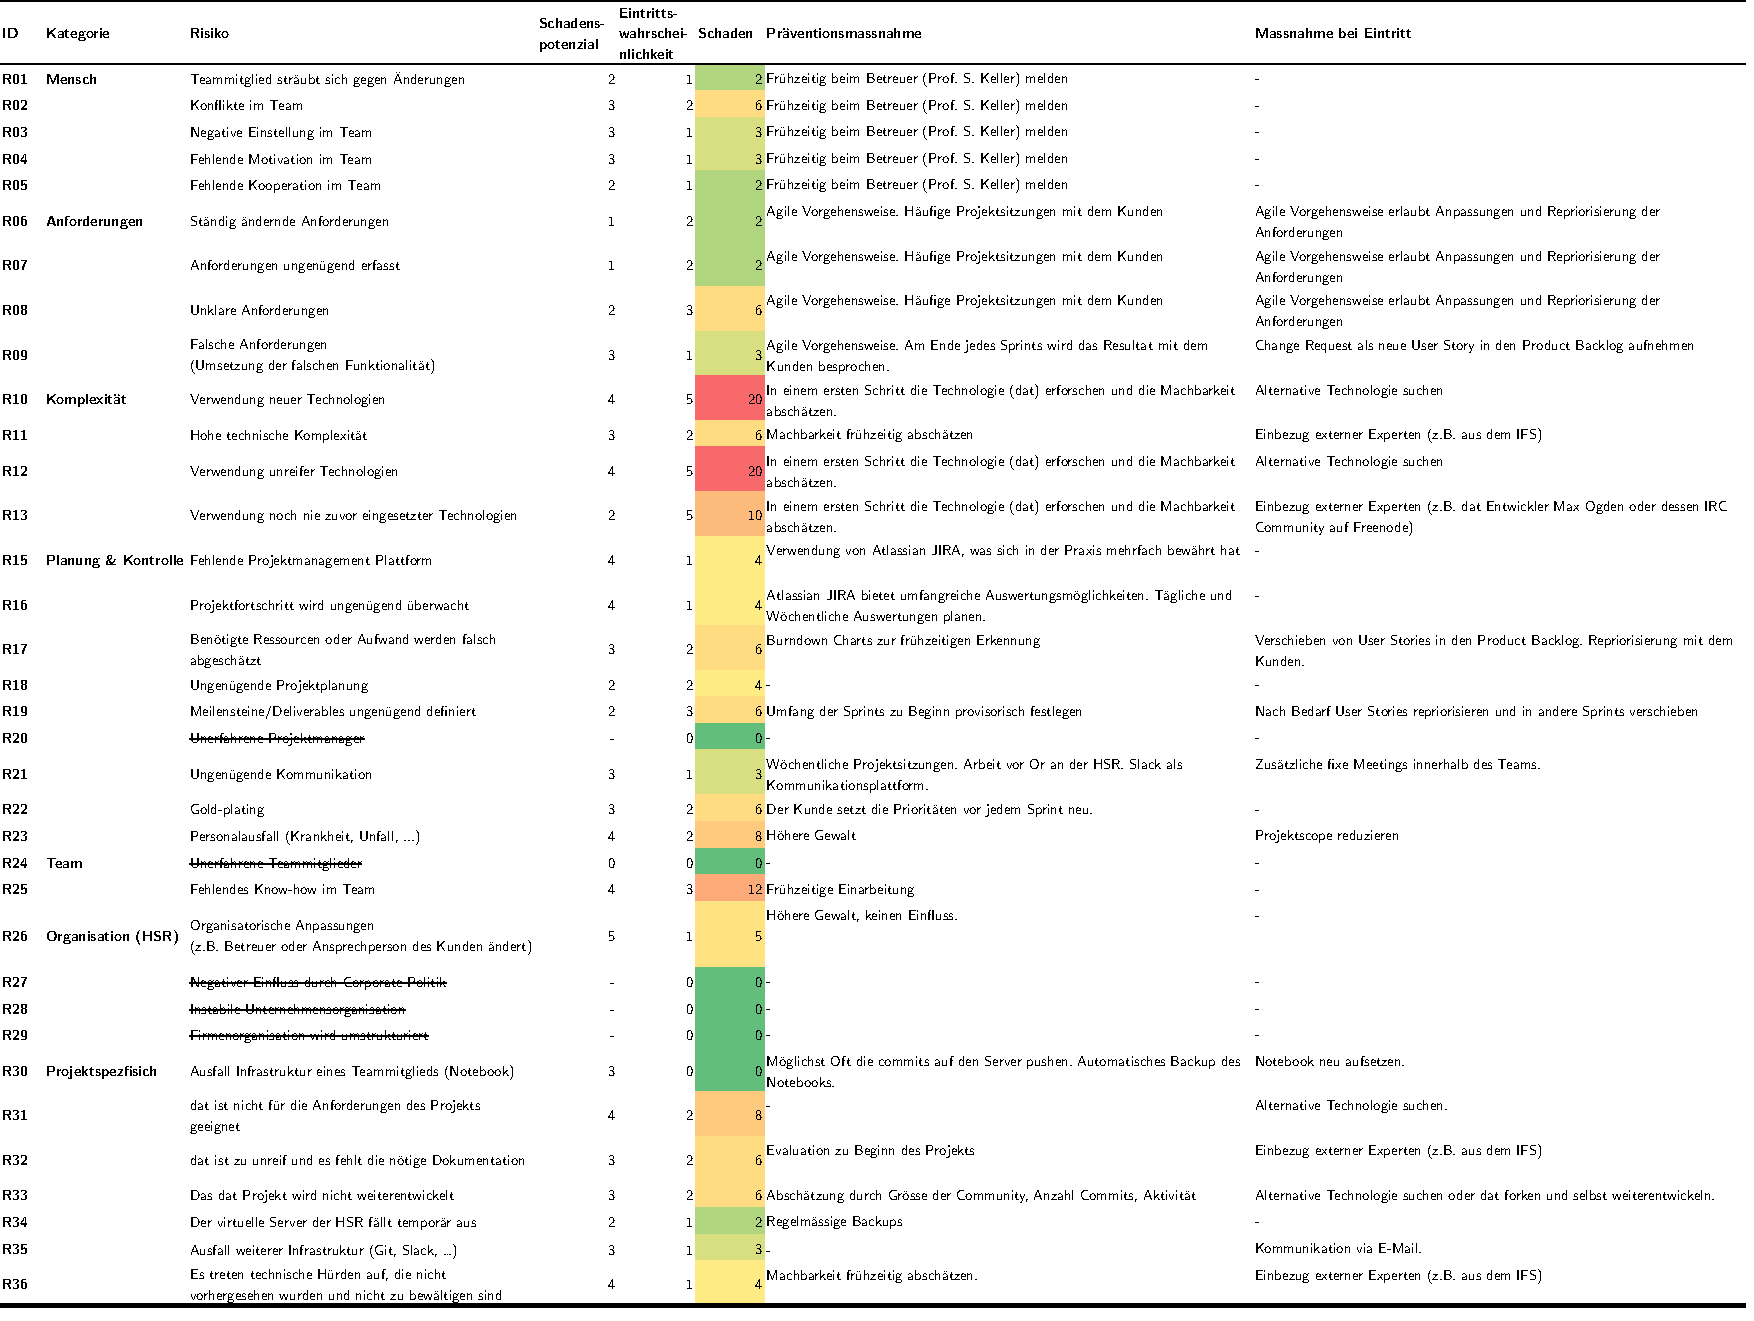
\includegraphics[height=.9\textheight,keepaspectratio]{risikoanalyse.pdf}
		\caption{Alle berücksichtigten Risiken}
		\label{tab:risikoanalyse}
	\end{table}
\end{landscape}



\section{Kritische Risiken}
Nach bzw. während der Einarbeitung in \gls{dat} wurde eine erste Abschätzung der Risiken vorgenommen. Alle irrelevanten oder ausschliessbare Risiken wurden dabei einer Eintrittswahrscheinlichkeit und Schadenspotenzial von 0 bewertet.

Nachfolgend werden die als besonders kritisch eingestuften Risiken sowie deren Massnahmen genauer beschrieben. Schon jetzt ist klar, dass das grösste Risiko das Projekt \gls{dat} selbst darstellt.


\newcommand{\projectrisk}[4]{
\begin{tabularx}{\linewidth}{lX}
	\toprule
	\textbf{Risiko} & #1\\
	\midrule
	\textbf{Titel} & #2\\
	\textbf{Beschreibung} & #3\\
	\textbf{Prävention/Massnahme} & #4\\
	\bottomrule
\end{tabularx}	
}


\projectrisk{R02}{Konflikte im Team}
{Das Projektteam kennt sich erst seit kurzem und hat davor noch nie zusammengearbeitet. Somit besteht ein erhöhten Risiko von Meinungsverschiedenheiten während des Projektverlaufs.}
{Frühzeitige Kontaktaufnahme mit dem Betreuer falls die Konflikte nicht intern gelöst werden können.}

\projectrisk{R10, R12, R13}{Verwendung neuer oder unreifer Technologien}
{Es werden unreife ``bleeding Edge'' Technologien verwendet welche die Entwicklung und Handhabung erheblich erschweren. Siehe auch \gls{dat}-spezifische Risiken R31, R32 und R33.}
{Es werden vor allem Technologien verwendet die dem Team bereits bekannt sind oder das Risiko durch eine Kurzevaluation reduziert.}

\projectrisk{R31}{\gls{dat} erfüllt nicht die Anforderungen}
{\gls{dat} und dessen Funktionalität ist nur sehr spärlich beschrieben. Selbst dem Auftraggeber ist der Umfang von \gls{dat} nicht vollständig bekannt. Es besteht das Risiko, dass \gls{dat} sich nicht für die Use Cases der Aufgabenstellung eignet.}
{Da es sich bei dieser Arbeit unter Anderem spezifisch um eine Evaluation von \gls{dat} und dessen Möglichkeiten handelt, ist eine Evaluation von alternativen Technologien zunächst zu vermeiden. Durch eine frühzeitige Einarbeitung in \gls{dat} mit kleineren Prototypen/Use Cases soll die Machbarkeit abgeschätzt werden.}


\projectrisk{R32}{\gls{dat} ist zu unreif. Fehlende Dokumentation.}
{\gls{dat} besitzt viele unbekannte Fehler und die Dokumentation ist unzureichend. Bereits während des ersten Sprints hat die spärliche Dokumentation von \gls{dat} zu Bedenken im Team geführt.}
{Dasselbe wie bei R31}


\projectrisk{R33}{\gls{dat} wird nicht weiterentwickelt}
{Der Kernentwickler von \gls{dat} (Max Ogden) verliert das Interesse am Projekt und \gls{dat} wird auch nicht von der Community nicht weiterentwickelt.}
{Abschätzung des Risikos durch die Aktivitäten der Entwickler sowie der grösse der Community. Da \gls{dat} Grundsätzlich durch die Aufgabenstellung vorgegeben ist, kann dieses Risiko nicht vermieden werden.}


\section{Risikoüberwachung}

Die Risiken wurden während des gesamten Projektverlaufs periodisch überwacht und Änderungen entsprechend protokolliert. Idealerweise sollten die Risiken über Zeit hinweg sinken.

\subsection{1. März 2015}

Wie sich herausgestellt hat, ist \gls{dat} noch weit davon entfernt um es produktiv Verwenden zu können. Ständige API Änderungen und fehlende Dokumentation machen es zu einem untragbaren Risiko. In \vref{dec:dat:fazit} wurde gegen den Einsatz von \gls{dat} Entschieden und somit die Risisken R31 bis R33 eliminiert.



\chapter{Entwicklungsumgebung und Infrastruktur}
In diesem Kapitel wird die Entwicklungsumgebung inkl. verwendete Tools beschrieben. \cref{fig:pm:entwicklungsumgebung} zeigt eine Übersicht der Entwicklungsumgebung und den groben Prozess.

\begin{figure}[H]
	\centering
	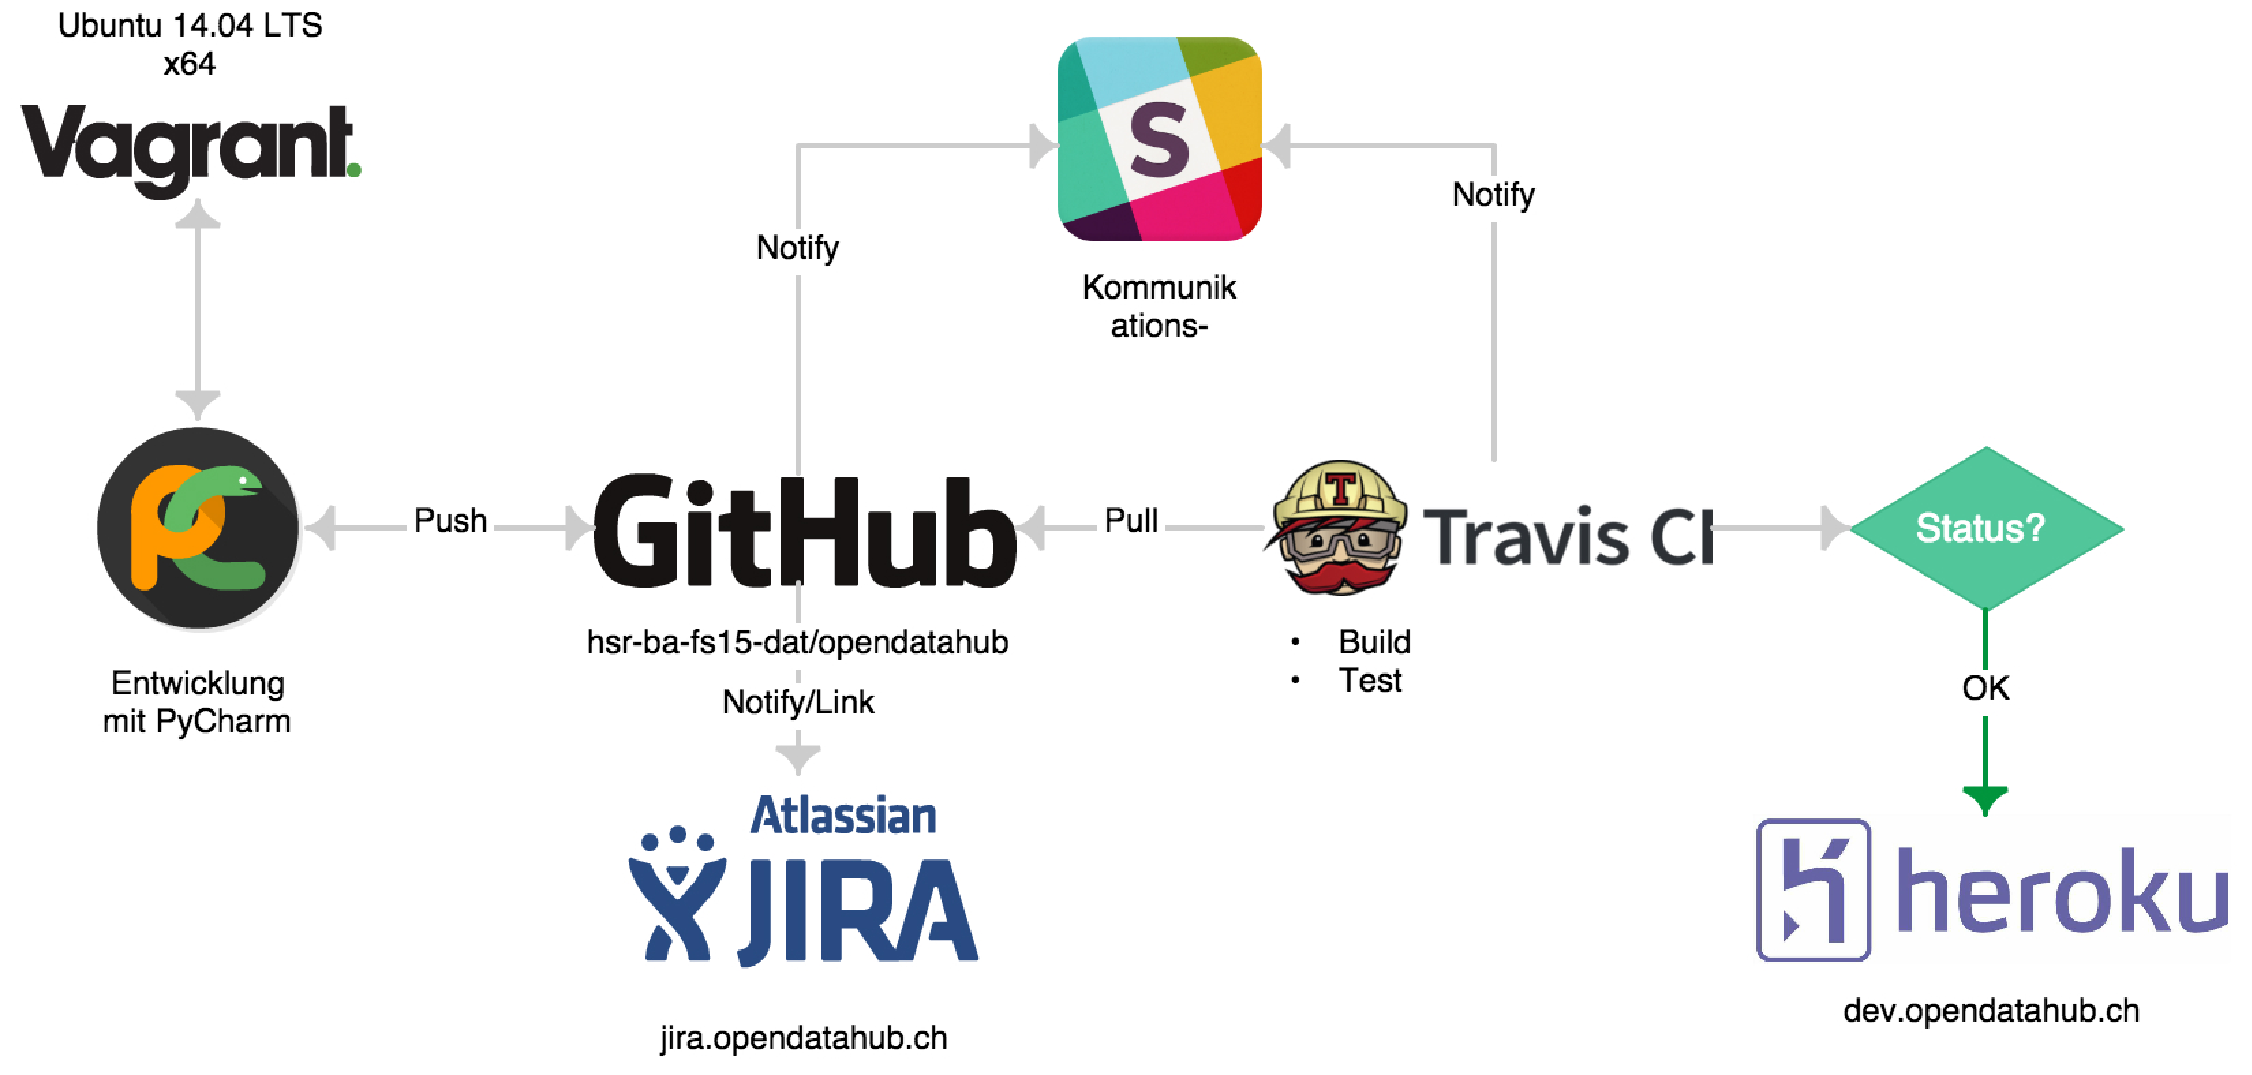
\includegraphics[width=\linewidth]{fig/entwicklungsumgebung}
	\caption{Entwicklungsumgebung}
	\label{fig:pm:entwicklungsumgebung}
\end{figure}

\section{IDE}
\xxx[more, why? pros/cons, use decision box?]
\begin{decision}{IDE}
	Als IDE wurde JetBrains PyCharm verwendet. Sämtliche Mitglieder waren bereits mit dieser IDE vertraut und die neuen Lizenzbestimmungne von JetBrains liessen eine kostenlose Nutzung der professionellen Version zu.

\end{decision}
\section{SCM}
\xxx[more, why? pros/cons, use decision box?]
Als \gls{scm} wurden GitHub Repositories innerhalb einer eigenen GitHub Organisation ``hsr-ba-fs15-dat'' verwendet.


\section{Projektmanagement}

Zur Planung der Ressourcen und Zeit sowie Zuständigkeiten der Tasks wurde das kommerzielle Tool Atlassian Jira verwendet. Jira ist kompatibel mit Agilen Vorgehensweisen, insbesondere Scrum und erlaubt mit dessen intuitivem User Interface die Planung von Sprints sowie eine Fortschrittsüberwachung mittels Burndown Charts. \cref{fig:pm:jira-agile} zeigt das sogenannte Agile Board im ``Work'' Modus während eines Sprints. Die Kopplung von Jira mit GitHub bietet mit der Verwendung von sog. Smart Commits\footnote{Beispiel: ``DAT-18 added project risks \#time 3h \#comment first draft''\newline\url{https://confluence.atlassian.com/display/FISHEYE/Using+smart+commits}} eine noch komfortablere Möglichkeit um Aufwände zu verbuchen oder Tasks zu kommentieren oder schliessen.

\begin{figure}[H]
	\centering
	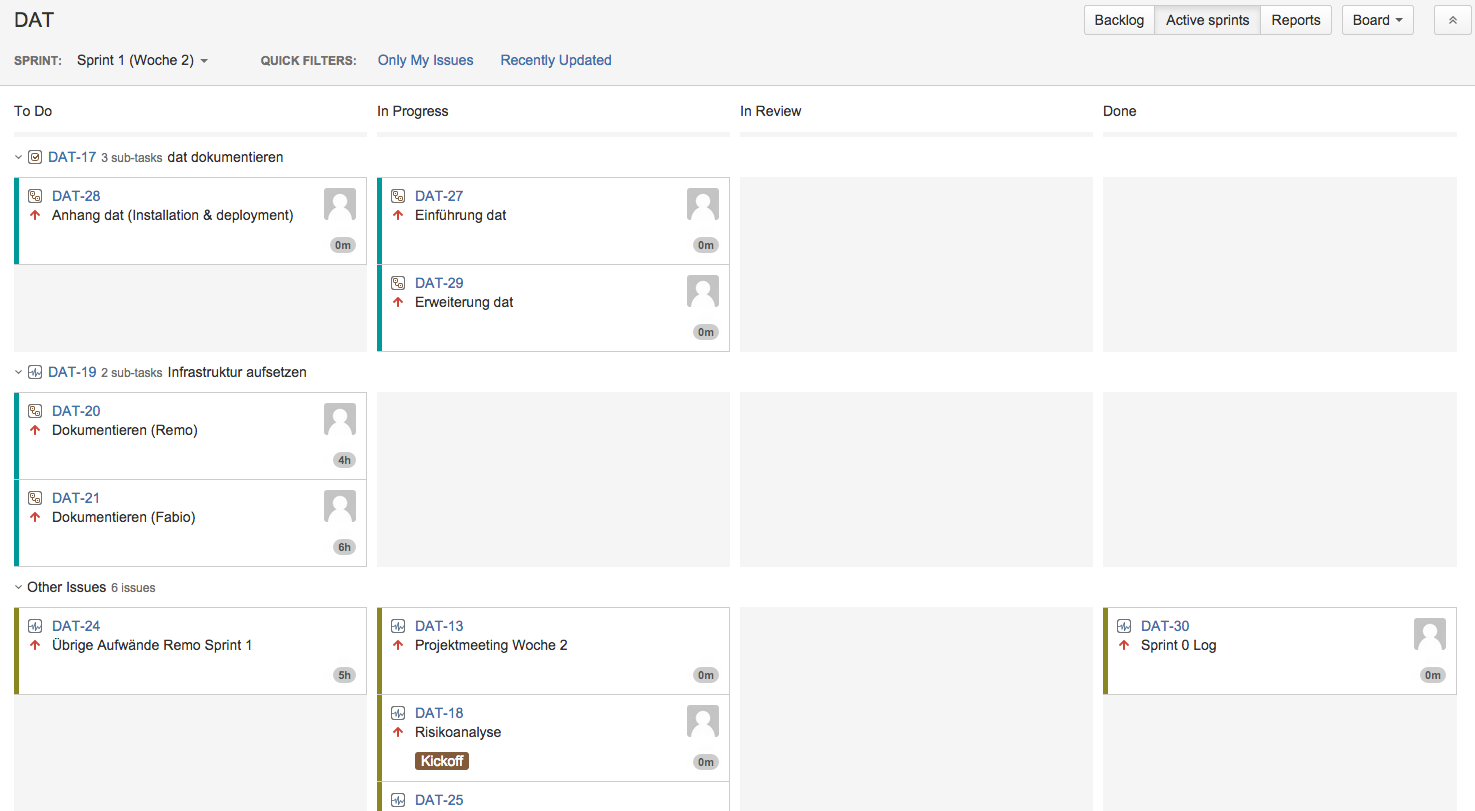
\includegraphics[width=0.95\textwidth]{fig/jira-agile}
	\caption{Jira Agile Board}
	\label{fig:pm:jira-agile}
\end{figure}

Jira wurde auf einer virtuellen Maschine der \acs{hsr} betrieben und dessen Daten täglich und automatisiert via cronjob gesichert.


\section{Kommunikation}
Bei der Durchführung der Bachelorarbeit \gls{dat} wollten wir auf die Kommunikation per E-Mail verzichten. Das Team hat sich mittels \purl{http://slack.com} ausgetauscht sowie als zur Protokollierung von Sitzungen, Weblinks und weitere Informationen verwendet. Slack bietet Team-Kommunikation auf hohem Niveau, mit der Möglichkeit Services wie GitHub, Jira, Travis-CI, E-Mails usw.\footnote{\url{https://slack.com/integrations}} zu integrieren. So konnte an einem zentralen Ort Bezug auf Commits, E-Mails vom Betreuer und Failing-Builds genommen werden. Durch die Verwendung eines dedizierten Tools zur Kommunikation konnte das E-Mail Postfach von Bachelor relevanten Themen freigehalten und direkten Bezug auf konkrete Ereignisse genommen werden.

\begin{figure}[H]
	\centering
	\begin{subfigure}{0.49\textwidth}
		\centering
		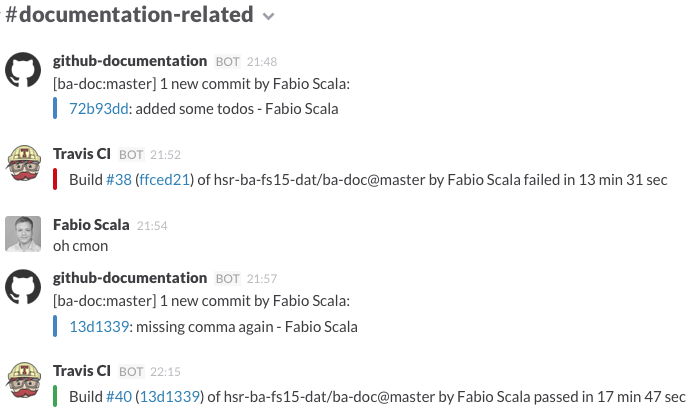
\includegraphics[width=\linewidth]{fig/slack-git-travis}
		\caption{Git und Travis}
		\label{fig:pm:slack-git-travis}
	\end{subfigure}
	\begin{subfigure}{0.49\textwidth}
		\centering
		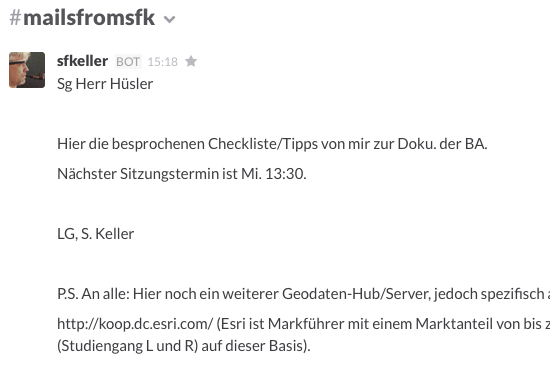
\includegraphics[width=\linewidth]{fig/slack-email}
		\caption{Automatische E-Mail Weiterleitung}
		\label{fig:pm:slack-email}
	\end{subfigure}
	\caption{Slack Screenshots}
	\label{fig:pm:slack}
\end{figure}


\section{Integrationsumgebung}
Die Applikation wird nach jedem erfolgreichen Build von Travis auf Heroku deployed. Die Integrationsinstanz dient zu Demozwecken an Sitzungen und stellt zudem sicher, dass die Webapplikation auch im Kompilierten\footnote{Transpilierung von TypeScript sowie Konkatentierung und ``Minification'' aller Ressourcen} funktioniert.


\chapter{Qualitätsmanagement}

\section{Reviews}

Um die Qualität der umgesetzten Tasks zu erhöhen und sicherzustellen wurde ein Review-Prozess eingesetzt. Jeder Task darf erst abgeschlossen werden, wenn ein anderes Teammitglied das Resultat grob angeschaut und für gut befunden hat. Um diesen Prozess einzuhalten wurde ein eigener Jira-Workflow verwendet.

\begin{figure}
\centering
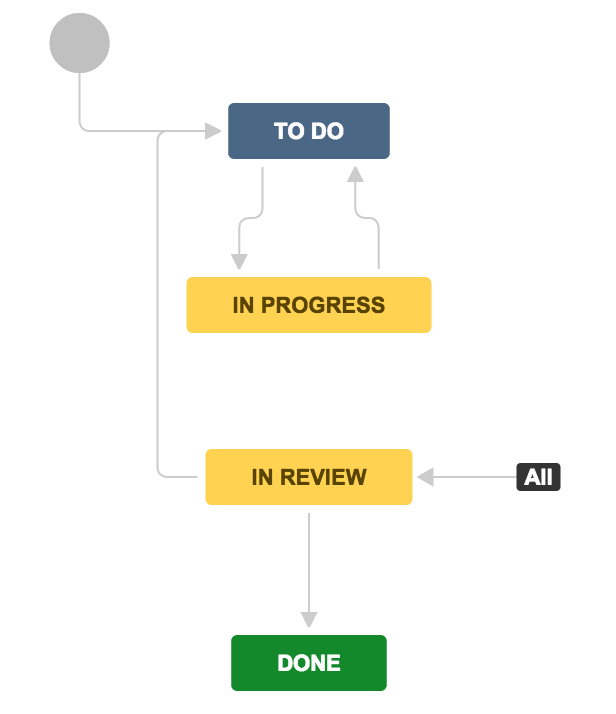
\includegraphics[width=0.7\linewidth]{fig/jira-workflow}
\caption{Jira Review-Workflow}
\label{fig:jira-workflow}
\end{figure}

Der in \cref{fig:jira-workflow} dargestellte Prozess stellt sicher, dass alle Tasks erst in den Review Status versetzt werden müssen. Von diesem Status aus kann der Task entweder durch den Reviewer geschlossen oder zurück in den Status ``To Do'' versetzt werden, wobei bei letzterem der Tasks automatisch dem ursprünglichen Teammitglied zugewiesen wird.


\section{Programmierrichtlinien}
Jeder Entwickler hat seine eigenen Vorstellungen davon wie Programmcode aussehen soll bzw. welche Richtlinien\footnote{Namenskonventionen, Modularität, \dots} bei der Entwicklung einzuhalten sind. Aus diesem Grund wurden frühzeitig Programmierrichtlinien inkl. Coding Style Guidelines bestimmt und mittels Entwicklungsumgebung\footnote{PyCharm von JetBrains (IntelliJ IDEA)} sowie Build-Server forciert.


\subsection{Python}
Für den Python Quellcode wurden die in der Python Community verbreiteten \gls{pep8} Richtlinien angewendet. Die einzige Ausnahme stellt hierbei eine Zeilenlänge von 120 statt den nur 80 Zeichen dar. Die \gls{pep8} Regeln werden teilweise durch die verwendete Entwicklungsumgebung sowie Flake8\footnote{\url{http://flake8.readthedocs.org}} und PyLint\footnote{\url{http://www.pylint.org/}} auf dem \gls{ci} Server streng erzwungen. Bei Verstoss versagt der Build und der Entwickler wird Benachrichtigt. Ein Beispiel-Output auf dem Build-Server sieht folgendermassen aus:

\begin{src}{console}
[INFO]  Executing flake8 on project sources.
[WARN]  flake8: src/main/python/authentication/tests.py:5:9: W292 no newline at end of file
[WARN]  flake8: src/main/python/authentication/tests.py:1:1: F401 'TestCase' imported but unused
[WARN]  flake8: src/main/python/authentication/admin.py:1:1: F401 'admin' imported but unused
[WARN]  flake8: src/main/python/opendatahub/urls.py:8:1: F401 'IndexView' imported but unused
------------------------------------------------------------
BUILD FAILED - flake8 found 4 warning(s)
\end{src}


\subsection{TypeScript}
Zur Formatierung des Quellcodes wurden die Standardregeln der Entwicklungsumgebung angewendet. Diese sind unter \path{opendatahub/idea/settings.jar} abgelegt. Auch hier wurde zur Prüfung und Einhaltung von TypeScript-spezifischen Regeln ein Linter (tslint) verwendet und mittels Build-Server erzwungen. Die Regeln sind in \path{opendatahub/src/main/webapp/tslint.json} konfiguriert. Da eine Typisierung in TypeScript optional ist, gilt der Grundsatz ``dort wo es Sinn macht'', das heisst konkret
\begin{itemize}
\item alle Variablen die ein TypeScript Interface besitzen (z.B. AngularJS Services),
\item alle public Funktionen und Methoden die auch exportiert werden und somit irgendwo Wiederverwendung finden sowie deren Attribute.
\end{itemize}

Nicht zu annotieren sind inline Lambda-Funktionen ausser deren Parameter sofern ein bestehendes Interface existiert. Ein Beispiel-Output von tslint sieht folgendermassen aus:

\begin{src}{console}
Running "tslint:files" (tslint) task
app/scripts/app.config.ts[2, 3]: comment must start with a space
app/scripts/app.config.ts[21, 3]: comment must start with a space
app/scripts/app.config.ts[21, 8]: file should end with a newline
app/scripts/app.ts[37, 11]: comment must start with lowercase letter
app/scripts/app.ts[5, 9]: unused variable: 'openDataHu
app/scripts/auth/controllers/account-settings.controller.ts[30, 15]: comment must start with lowercase letter
app/scripts/auth/controllers/account-settings.controller.ts[34, 19]: comment must start with a space
7 errors in 3 files
Warning: Task "tslint:files" failed. Use --force to continue.
Aborted due to warnings.
------------------------------------------------------------
BUILD FAILED - Errors while running grunt, see /home/travis/build/hsr-ba-fs15-dat/opendatahub/target/reports/grunt.err
\end{src}


\subsection{AngularJS}
Bei AngularJS gibt es eine Vielzahl von Möglichkeiten ein und dasselbe zu erreichen. Aus diesem Grund ist es umso wichtiger sich auf bestimmte Vorgehensweisen bei der Entwicklung mit AngularJS zu einigen. Grundsätzlich gelten die mittlerweile etablierten und nahezu offiziellen AngularJS Richtlinien und Best Practices von ``John Papa''\cite{angular-styleguide}. Die Richtlinien sind auf JavaScript ausgelegt. Da wir TypeScript verwenden sind nur diejenigen anzuwenden die auch im TypeScript Kontext zutreffen bzw. noch Sinn machen. Besonders zu beachten sind folgende Regeln:

\begin{itemize}
	\item Verwendung der ``controller as'' Syntax um Scope-Vererbung zu vermeiden
	\item DOM Manipulationen finden ausschliesslich in AngularJS Direktiven statt
	\item Single Responsibility Priciple \textendash\ Eine Klasse/Service/Controller pro Datei mit Ausnahme von kleinen ``Sub-Controllern'' die zu einem anderen gehören oder nicht exportierte (private) Klassen.
\end{itemize}

Es wurden eigene TypeScript ``New File'' IntelliJ Templates für AngularJS Services, Controller und Direktiven erstellt und stellen sicher, dass jeder Entwickler immer wieder dieselbe Grundstruktur verwendet. Diese sind unter \path{opendatahub/idea/settings.jar} abgelegt.



\subimport{sprints/}{sprints.tex}


